\documentclass[hyperref={unicode}]{beamer}

\usepackage[utf8]{inputenc}
\usepackage[english]{babel}
\usepackage[T1]{fontenc}
\usepackage{csquotes,lmodern,silence}
\usepackage{marvosym}
\usepackage{textpos}
\usepackage{graphbox}
% \usepackage[labelformat=simple]{caption}


% \DeclareGraphicsExtensions{.pdf,.png}


%
% Choose how your presentation looks.
%
% For more themes, color themes and font themes, see:
% http://deic.uab.es/~iblanes/beamer_gallery/index_by_theme.html
%
\mode<presentation> {
	\usetheme{Berkeley}      % or try Darmstadt, Madrid, Warsaw, ...
	\usecolortheme{wolverine} % or try albatross, beaver, crane, ...
	\usefonttheme{default}  % or try serif, structurebold, ...
	\setbeamertemplate{navigation symbols}{}
	\setbeamertemplate{caption}[numbered]
% 	\setbeamertemplate{caption}{\raggedright\insertcaption\par}[numbered]
	% Numbered bibiolgraphy items
%	\setbeamertemplate{bibliography item}{\insertbiblabel}
	\setbeamertemplate{itemize item}{$\mbox{\Lightning}$}

	\setbeamerfont{section in sidebar}{size=\fontsize{11}{11}\selectfont}
	\setbeamerfont{subsection in sidebar}{size=\fontsize{7}{7}\selectfont}
	\setbeamerfont{subsubsection in sidebar}{size=\fontsize{4}{4}\selectfont}
}

\addto\captionsenglish{%
	\renewcommand{\figurename}{Obrázok}
}

%\usepackage[style=numeric,backend=biber]{biblatex}

%\WarningFilter{biblatex}{Patching footnotes failed}

% Remove small caps warning
%\renewcommand\mkbibacro[1]{{\footnotesize\MakeUppercase{#1}}}

%\addbibresource{bibliography.bib}
\graphicspath{{figures/}}

\title[DP prezentácia]{Viacúčelový systém merania elektrického výkonu dodávaný elektrickými zásuvkami}
\author{Peter Babič}
\institute{Technická Univerzita v Košiciach \\ Počítačové Modelovanie, Ing.}
\date{24.05.2016}

\begin{document}

\addtobeamertemplate{frametitle}{}{%
	\begin{textblock*}{1cm}(.55\textwidth,-1.45cm)
		
\includegraphics[height=1.25cm,width=1.25cm]{logo-tu}
	\end{textblock*}
	\begin{textblock*}{1cm}(.70\textwidth,-1.45cm)
		
\includegraphics[height=1.25cm,width=1.25cm]{logo-fei}
	\end{textblock*}
	\begin{textblock*}{1cm}(.85\textwidth,-1.45cm)
		
\includegraphics[height=1.25cm,width=1.75cm]{logo-kmti}
	\end{textblock*}
}



\section{Úvod}
\label{sec:Úvod}

\subsection{Predhovor}
\label{sub:Predhovor}

\begin{frame}{\phantom{A}}
	\maketitle
\end{frame}



\subsection{Podnety}
\label{sub:Podnety}

\begin{frame}{Podnety práce}
	\begin{itemize}
		\item Môžeme si dovoliť plytvať elektrickou energiou?
		\item Prečo merať výkon už pri zásuvke?
		\item Čo chýba meračom už zavedeným na trhu?
	\end{itemize}

	\def \myGraphicsHeight {4.5cm}
	\begin{figure}[htp]
		\centering
		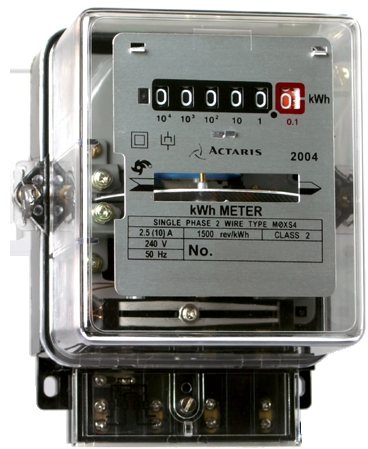
\includegraphics[height=\myGraphicsHeight]{analog-power-meter}
		\hspace{1cm}
		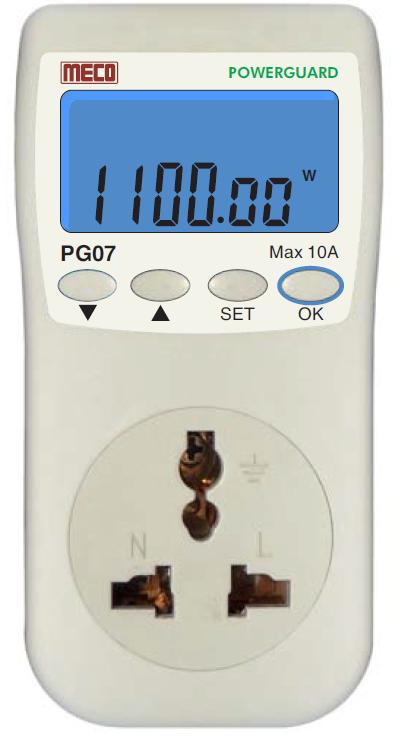
\includegraphics[height=\myGraphicsHeight]{digital-plug-meter}
		\caption{Merač v rozvodovej skrini a zásuvkový merač}
	\end{figure}

\end{frame}



\section{Riešenie}
\label{sec:Riešenie}

\subsection{Návrh}
\label{sub:Návrh}

\def \myGraphicsHeight {2.5cm}
\begin{frame}{Návrh riešenia}
	\begin{figure}[htp]
		\centering
		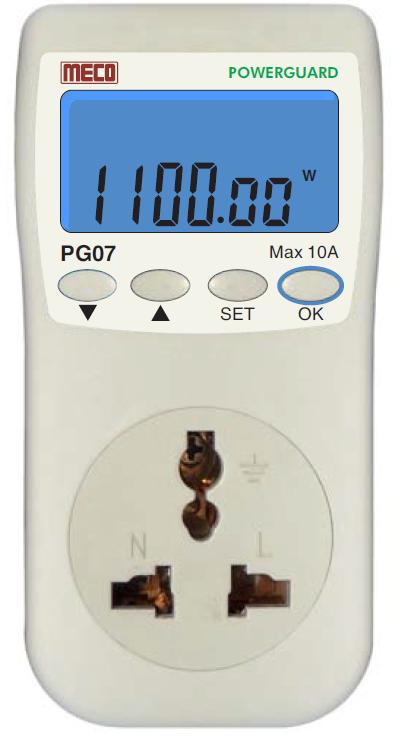
\includegraphics[align=c,height=\myGraphicsHeight]{digital-plug-meter}
		{\Huge +}
		
\includegraphics[align=c,height=\myGraphicsHeight]{logo-wifi}
		{\Huge +}
		
\includegraphics[align=c,height=\myGraphicsHeight]{cloud-computing}
		\caption{Recept na diplomovú prácu}
	\end{figure}
\end{frame}



\subsection{Vizualizácia}
\label{sub:Vizualizácia}

\def \myGraphicsHeight {.60\paperheight}
\begin{frame}{Vizualizácia návrhu}
	\begin{figure}[htp]
		\centering
		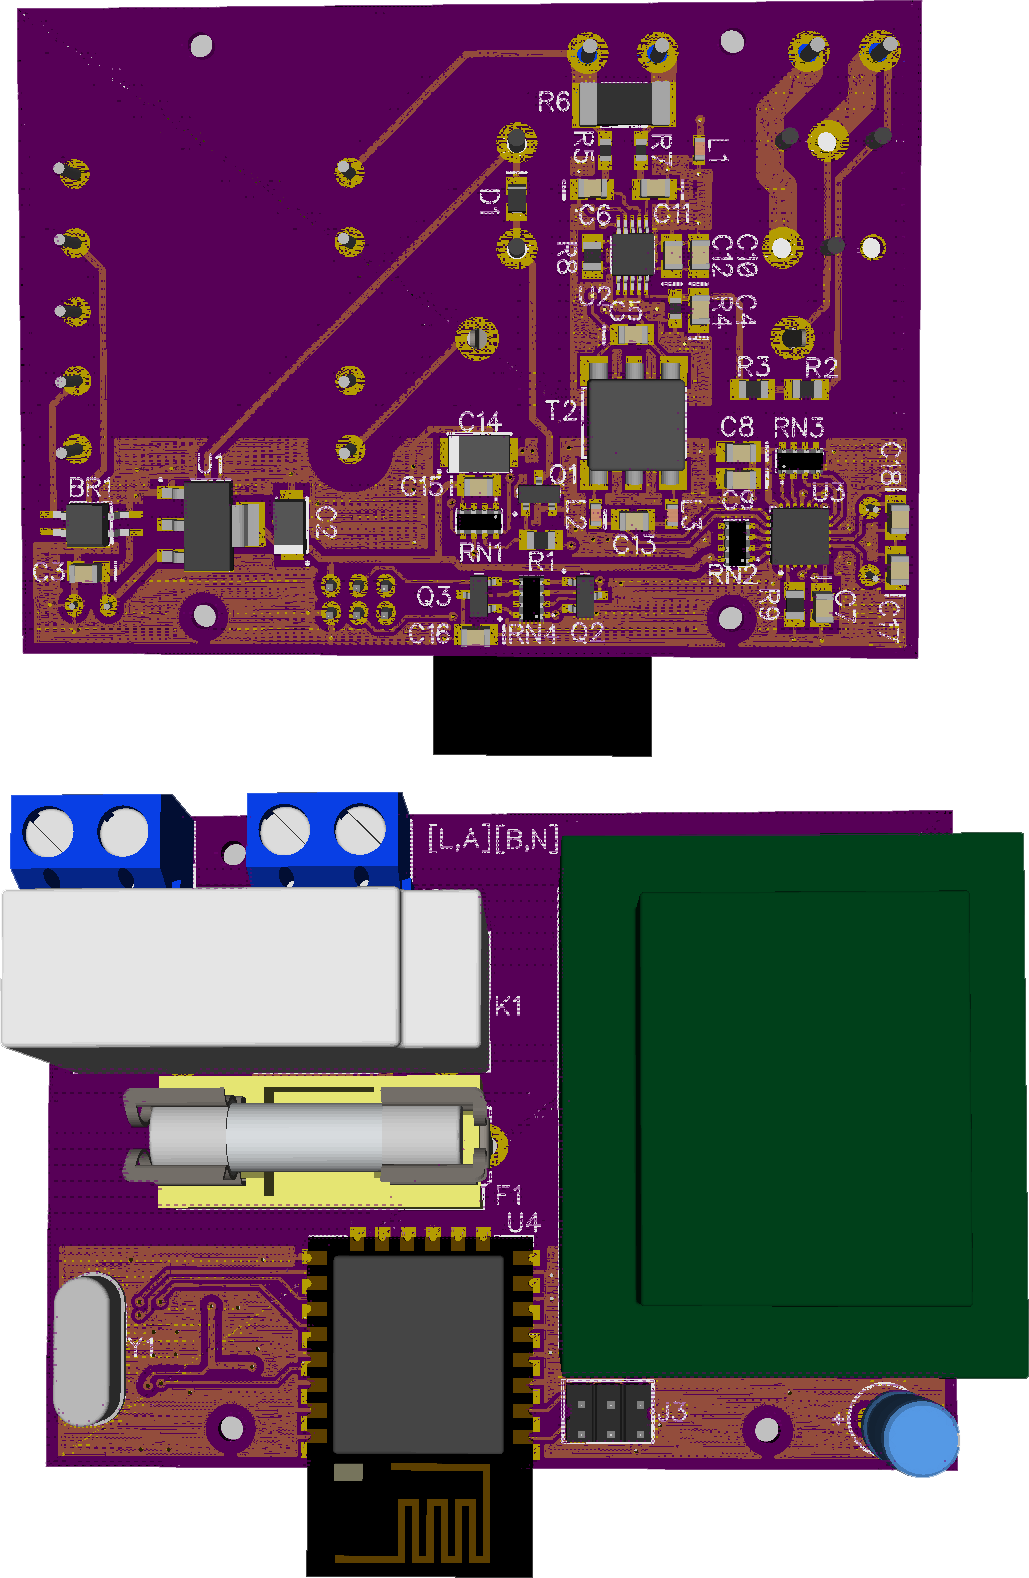
\includegraphics[height=\myGraphicsHeight]{visualisation}
		% \hspace{1cm}
		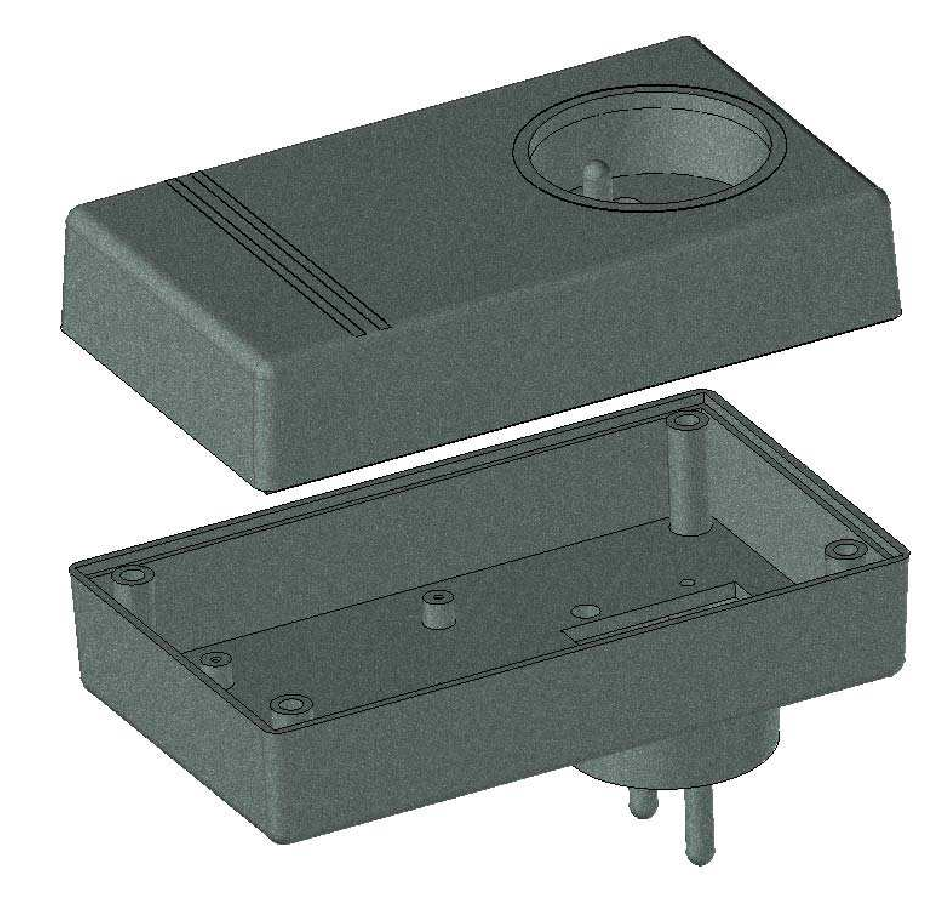
\includegraphics[height=\myGraphicsHeight]{enclosure}
		\caption{Vizualizácia plošného spoja a krabičky pred zhotovením}
	\end{figure}
\end{frame}



\subsection{Dáta}
\label{sub:Dáta}

\begin{frame}{Namerané dáta}
	\begin{figure}[htp]
		\centering
		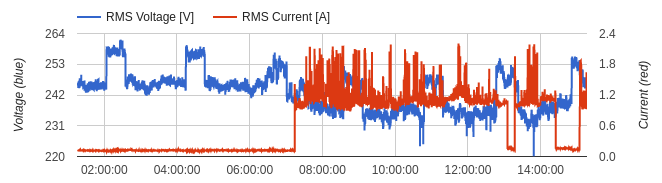
\includegraphics[width=1\linewidth]{plot-preview}
		\caption{Web server zobrazujúci namerané dáta}
	\end{figure}
\end{frame}



\section{Otázky}
\label{sec:Otázky}

\subsection{Vedúci DP}
\label{sub:Vedúci}

\begin{frame}{Otázka vedúceho DP}
	\begin{block}{Znenie}
		V kapitole 7.2 ste popisovali príklad merania, kde ste na server posielali údaje každých 10s. V akom najkratšom časovom intervale by bolo možné posielať namerané dáta pomocou vami vytvoreného meracieho systému?
	\end{block}

	\begin{equation*}
		\frac{100\;\text{zápisov}}{15\;\text{min}} = \frac{100\;\text{zápisov}}{900\;\text{sec}} = \frac{1\;\text{zápis}}{9\;\text{sec}}\;\text{max} \cong \frac{1\;\text{zápis}}{10\;\text{sec}}
	\end{equation*}
\end{frame}



\subsection{Odpoveď}
\label{sub:Odpoveď}

\begin{frame}{Otázka vedúceho DP}
	\begin{equation*}
		\frac{1767\,\text{vzoriek/sec}}{400\,\text{vzoriek/interval}} = \frac{400}{1767}\,\text{Hz} = 226.3723\times 10^{-3}\,\text{sec}\cong 224\,\text{ms}
	\end{equation*}

	\begin{block}{Odpoveď}
		Použitím vlastného serveru sa odstráni limit 100 zápisov v rozmedzí 15 minút. Pri použití WebSockets spojenia merača so serverom, je možné \textbf{teoretické maximum} odosielania dát hneď ako sú dostupné, teda každých 224 ms.
	\end{block}
\end{frame}



\subsection{Záver}
\label{sub:Záver}

\begin{frame}{Záver prezentácie}
	\centering
	{\Large Ďakujem za Vašu pozornosť.\\
	\vspace{1cm}
	(priestor pre Vaše otázky)}
\end{frame}



\end{document}
